\documentclass[a4paper]{article}

\usepackage[czech]{babel} %https://github.com/michal-h21/biblatex-iso690
\usepackage[
   backend=biber      % if we want unicode 
  ,style=iso-numeric % or iso-numeric for numeric citation method          
  ,babel=other        % to support multiple languages in bibliography
  ,sortlocale=cs_CZ   % locale of main language, it is for sorting
  ,bibencoding=UTF8   % this is necessary only if bibliography file is in different encoding than main document
]{biblatex}

\usepackage[utf8]{inputenc}
\usepackage{fancyhdr}
\usepackage{amsmath}
\usepackage{amssymb}
\usepackage[left=2cm,right=2cm,top=2.5cm,bottom=2.5cm]{geometry}
\usepackage{graphicx}
\usepackage{pdfpages}
\usepackage{url}

\usepackage{siunitx}
\sisetup{locale = DE}  %, separate-uncertainty = true    kdybych chtel +/-

\usepackage{float}
\newfloat{graph}{htbp}{grp}
\floatname{graph}{Graf}
\newfloat{tabulka}{htbp}{tbl}
\floatname{tabulka}{Tabulka}

\renewcommand{\thefootnote}{\roman{footnote}}

\pagestyle{fancy}
\lhead{Praktikum III - (2) Měření parametrů zobrazovacích soustav}
\rhead{Vladislav Wohlrath}
\author{Vladislav Wohlrath}

\bibliography{source}

\begin{document}

\begin{titlepage}
\includepdf[pages={1}]{./graficos/302-tit.pdf}
\end{titlepage}

\section*{Pracovní úkoly}
\begin{enumerate}
\item ÚKOLY
\end{enumerate}

%Teoretická část
\section*{Teoretická část}

%Podmínky a měřící přístroje
\section*{Podmínky a použité přístroje}

%Výsledky měření
\section*{Výsledky měření}
Jako tenkou čočku jsme použili čočku označenou číslicí 5.
Změřili jsme polohu čočky a velikost obrazu pro 5 různých hodnot $D$. Změřené hodnoty jsou v tabulce \ref{t:oh}. Velikost předmětu byla $Y=\SI{10}{\mm}$. $f_B$ značíme ohniskovou vzdálenost vypočtenou z \eqref{e:bessel} Besselovou metodou.
Standardní odchylku určení polohy čočky, ve které byl obraz ostrý, odhadujeme na \SI{2}{\mm}. Standardní odchylku určení velikosti obrazu odhadujeme na \SI{0.3}{\mm}.

Hodnoty $f_B$ se příliš neliší, takže z nich určíme střední hodnotu a standardní odchylku, ve které zohledníme chyby přímo měřených veličin
\begin{equation*}
f_B=\SI{10.82(10)}{\cm}
\end{equation*}

Z hodnot v tabulce \ref{t:oh} jsme spočítali z \eqref{e:dvojizvetseni} ohniskovou vzdálenost $f_a$ resp. $f_{\apr}$ metodou dvojího zvětšení pro variaci předmětové resp. obrazové vzdálenosti. Vzorec \eqref{e:dvojizvetseni} je citlivý na blízké hodnoty argumentů $a$, $\apr$ nebo $\beta$. Proto jsme vybrali jen několik měření, ve kterých se příslušné argumenty dostatečně liší. Vybraná měření jsou uvedeny v tabulce \ref{t:dvoji}. Výsledné hodnoty jsou
\begin{equation*}
f_{a} = \SI{10.2(10)}{\cm} \qquad \qquad f_{\apr}=\SI{10.4(1)}{\cm} \,.
\end{equation*}

\begin{tabulka}[htbp]
\centering
\begin{tabular}{cc|cccc|c}
$D$ (\si{\cm}) & $\Delta$ (\si{\cm}) & $a$ (\si{\cm}) & $\apr$ (\si{\cm}) & $\Ypr$ (\si{\mm}) & $ \beta$ & $f_B$ (\si{\cm}) \\ \hline \hline
\multirow{2}{*}{54,0} & 24,1 & 38,5 & 15,5 & 3,7 & 0,37 & 10,81 \\ 
 &  & 14,4 & 39,6 & 26,5 & 2,65 &  \\ \hline
\multirow{2}{*}{114,0} & \multirow{2}{*}{89,3} & 11,7 & 102,3 & 87,3 & 8,73 & \multirow{2}{*}{10,81} \\ 
 &  & 101,0 & 13,0 & 1,2 & 0,12 &  \\ \hline
\multirow{2}{*}{94,0} & \multirow{2}{*}{68,9} & 12,0 & 82,0 & 66,8 & 6,68 & \multirow{2}{*}{10,87} \\ 
 &  & 80,9 & 13,1 & 1,7 & 0,17 &  \\ \hline
\multirow{2}{*}{79,0} & \multirow{2}{*}{53,1} & 65,5 & 13,5 & 2,0 & 0,20 & \multirow{2}{*}{10,83} \\ 
 &  & 12,4 & 66,6 & 53,4 & 5,34 &  \\ \hline
\multirow{2}{*}{64,0} & \multirow{2}{*}{36,7} & 49,8 & 14,2 & 2,6 & 0,26 & \multirow{2}{*}{10,74} \\ 
 &  & 13,1 & 50,9 & 37,7 & 3,77 &  \\ \hline
\multirow{2}{*}{46,0} & \multirow{2}{*}{12,3} & 16,2 & 29,8 & 26,7 & 2,67 & \multirow{2}{*}{10,68} \\ 
 &  & 28,5 & 17,5 & 5,6 & 0,56 &  \\ 
\end{tabular}
\caption{Měření ohniskové vzdálenosti Besselovou metodou}
\label{t:oh}
\end{tabulka}

\begin{tabulka}[htbp]
\centering
\begin{tabular}{cc|cc|cc|cc}
$a_1$ (\si{\cm}) & $a_2$ (\si{\cm}) & $\apr_1$ (\si{\cm}) & $\apr_2$ (\si{\cm}) & $\beta_1$ & $\beta_2$ & $f_{a}$ (\si{\cm}) & $f_{\apr}$ (\si{\cm}) \\ \hline
11,7 & 28,5 & 102,3 & 17,5 & 8,73 & 0,56 & \num{10,0(8)} & \num{10,38(1)} \\ 
11,7 & 12,4 & 102,3 & 66,6 & 8,73 & 5,34 & \num{9,6(30)} & \num{10,53(3)} \\ 
101,0 & 12,4 & 13,0 & 66,6 & 0,12 & 5,34 & \num{10,9(30)} & \num{10,27(2)} \\ 
12,4 & 49,8 & 66,6 & 14,2 & 5,34 & 0,26 & \num{10,2(14)} & \num{10,31(2)} \\ 
28,5 & 12,0 & 17,5 & 82,0 & 0,56 & 6,68 & \num{10,1(8)} & \num{10,54(1)} \\ 
38,5 & 12,0 & 15,5 & 82,0 & 0,37 & 6,68 & \num{10,4(10)} & \num{10,54(1)} \\ 
\end{tabular}
\caption{Měření ohniskové vzdálenosti metodou dvojího zvětšení}
\label{t:dvoji}
\end{tabulka}






Pro měření kulové vady jsme použili sadu mezikružných clon. Jako vzdálenost paprsku od optické osy $s$ považujeme podle zadání aritmetický průměr největšího a nejmenšího poloměru.
Změřené hodnoty jsou v tabulce \ref{t:kulvada} a zaneseny do grafu \ref{g:vada}.


Závislost $v(s)$ jsme nafitovali funkcí tvaru \eqref{t:kulvada} a dostali hodnoty
\begin{equation} \label{e:vysledky}
\begin{array}{rclrcl}
K_{V | a=\SI{30}{\cm}} & = & \SI{-39(2)}{\per\metre} \qquad \qquad & K_{V | a=\SI{60}{\cm}} & = & \SI{-19.7(3)}{\per\metre} \\
K_{P | a=\SI{30}{\cm}} & = &\SI{-58(3)}{\per\metre} \qquad \qquad & K_{P | a=\SI{60}{\cm}} & = & \SI{-48(2)}{\per\metre} \\
\end{array}
\end{equation}

\begin{tabulka}[htbp]
\centering
\begin{tabular}{c|cc|cc||cc|cc}
& \multicolumn{4}{c||}{$a = \SI{30}{\cm}$} & \multicolumn{4}{c}{$a = \SI{60}{\cm}$} \\
& \multicolumn{2}{c|}{vypuklá} & \multicolumn{2}{c||}{ploská} & \multicolumn{2}{c|}{vypuklá} & \multicolumn{2}{c}{ploská} \\
$s$ (\si{\mm}) & $\apr$ (\si{\cm}) & $v$ (\si{\cm}) & $\apr$ (\si{\cm}) & $v$ (\si{\cm}) & $\apr$ (\si{\cm}) & $v$ (\si{\cm}) & $\apr$ (\si{\cm}) & $v$ (\si{\cm}) \\ \hline
0,0 & 22,4 & --- & 23,0 & --- & 18,7 & --- & 19,8 & --- \\ 
7,5 & 22,2 & -0,2 & 22,9 & -0,1 & 18,6 & -0,1 & 19,6 & -0,2 \\ 
12,5 & 21,7 & -0,7 & 22,3 & -0,7 & 18,4 & -0,3 & 19,1 & -0,7 \\ 
17,5 & 21,3 & -1,1 & 21,2 & -1,8 & 18,1 & -0,6 & 18,4 & -1,4 \\ 
22,5 & 20,4 & -2,0 & 20,0 & -3,0 & 17,7 & -1,0 & 17,3 & -2,5 \\ 
\end{tabular}
\caption{Kulová vada tenké čočky. Vypuklá/ploská označuje, která strana čočky byla směrem k předmětu.}
\label{t:kulvada}
\end{tabulka}

\begin{graph}[htbp] 
\centering
% GNUPLOT: LaTeX picture with Postscript
\begingroup
  \makeatletter
  \providecommand\color[2][]{%
    \GenericError{(gnuplot) \space\space\space\@spaces}{%
      Package color not loaded in conjunction with
      terminal option `colourtext'%
    }{See the gnuplot documentation for explanation.%
    }{Either use 'blacktext' in gnuplot or load the package
      color.sty in LaTeX.}%
    \renewcommand\color[2][]{}%
  }%
  \providecommand\includegraphics[2][]{%
    \GenericError{(gnuplot) \space\space\space\@spaces}{%
      Package graphicx or graphics not loaded%
    }{See the gnuplot documentation for explanation.%
    }{The gnuplot epslatex terminal needs graphicx.sty or graphics.sty.}%
    \renewcommand\includegraphics[2][]{}%
  }%
  \providecommand\rotatebox[2]{#2}%
  \@ifundefined{ifGPcolor}{%
    \newif\ifGPcolor
    \GPcolortrue
  }{}%
  \@ifundefined{ifGPblacktext}{%
    \newif\ifGPblacktext
    \GPblacktextfalse
  }{}%
  % define a \g@addto@macro without @ in the name:
  \let\gplgaddtomacro\g@addto@macro
  % define empty templates for all commands taking text:
  \gdef\gplbacktext{}%
  \gdef\gplfronttext{}%
  \makeatother
  \ifGPblacktext
    % no textcolor at all
    \def\colorrgb#1{}%
    \def\colorgray#1{}%
  \else
    % gray or color?
    \ifGPcolor
      \def\colorrgb#1{\color[rgb]{#1}}%
      \def\colorgray#1{\color[gray]{#1}}%
      \expandafter\def\csname LTw\endcsname{\color{white}}%
      \expandafter\def\csname LTb\endcsname{\color{black}}%
      \expandafter\def\csname LTa\endcsname{\color{black}}%
      \expandafter\def\csname LT0\endcsname{\color[rgb]{1,0,0}}%
      \expandafter\def\csname LT1\endcsname{\color[rgb]{0,1,0}}%
      \expandafter\def\csname LT2\endcsname{\color[rgb]{0,0,1}}%
      \expandafter\def\csname LT3\endcsname{\color[rgb]{1,0,1}}%
      \expandafter\def\csname LT4\endcsname{\color[rgb]{0,1,1}}%
      \expandafter\def\csname LT5\endcsname{\color[rgb]{1,1,0}}%
      \expandafter\def\csname LT6\endcsname{\color[rgb]{0,0,0}}%
      \expandafter\def\csname LT7\endcsname{\color[rgb]{1,0.3,0}}%
      \expandafter\def\csname LT8\endcsname{\color[rgb]{0.5,0.5,0.5}}%
    \else
      % gray
      \def\colorrgb#1{\color{black}}%
      \def\colorgray#1{\color[gray]{#1}}%
      \expandafter\def\csname LTw\endcsname{\color{white}}%
      \expandafter\def\csname LTb\endcsname{\color{black}}%
      \expandafter\def\csname LTa\endcsname{\color{black}}%
      \expandafter\def\csname LT0\endcsname{\color{black}}%
      \expandafter\def\csname LT1\endcsname{\color{black}}%
      \expandafter\def\csname LT2\endcsname{\color{black}}%
      \expandafter\def\csname LT3\endcsname{\color{black}}%
      \expandafter\def\csname LT4\endcsname{\color{black}}%
      \expandafter\def\csname LT5\endcsname{\color{black}}%
      \expandafter\def\csname LT6\endcsname{\color{black}}%
      \expandafter\def\csname LT7\endcsname{\color{black}}%
      \expandafter\def\csname LT8\endcsname{\color{black}}%
    \fi
  \fi
  \setlength{\unitlength}{0.0500bp}%
  \begin{picture}(10204.00,6802.00)%
    \gplgaddtomacro\gplbacktext{%
      \csname LTb\endcsname%
      \put(814,704){\makebox(0,0)[r]{\strut{}-35}}%
      \csname LTb\endcsname%
      \put(814,1537){\makebox(0,0)[r]{\strut{}-30}}%
      \csname LTb\endcsname%
      \put(814,2371){\makebox(0,0)[r]{\strut{}-25}}%
      \csname LTb\endcsname%
      \put(814,3204){\makebox(0,0)[r]{\strut{}-20}}%
      \csname LTb\endcsname%
      \put(814,4037){\makebox(0,0)[r]{\strut{}-15}}%
      \csname LTb\endcsname%
      \put(814,4870){\makebox(0,0)[r]{\strut{}-10}}%
      \csname LTb\endcsname%
      \put(814,5704){\makebox(0,0)[r]{\strut{}-5}}%
      \csname LTb\endcsname%
      \put(814,6537){\makebox(0,0)[r]{\strut{} 0}}%
      \csname LTb\endcsname%
      \put(946,484){\makebox(0,0){\strut{} 0}}%
      \csname LTb\endcsname%
      \put(2718,484){\makebox(0,0){\strut{} 5}}%
      \csname LTb\endcsname%
      \put(4490,484){\makebox(0,0){\strut{} 10}}%
      \csname LTb\endcsname%
      \put(6263,484){\makebox(0,0){\strut{} 15}}%
      \csname LTb\endcsname%
      \put(8035,484){\makebox(0,0){\strut{} 20}}%
      \csname LTb\endcsname%
      \put(9807,484){\makebox(0,0){\strut{} 25}}%
      \put(176,3620){\rotatebox{-270}{\makebox(0,0){\strut{}$v$ (\si{\mm})}}}%
      \put(5376,154){\makebox(0,0){\strut{}$s$ (\si{\mm})}}%
    }%
    \gplgaddtomacro\gplfronttext{%
      \csname LTb\endcsname%
      \put(3190,1537){\makebox(0,0)[r]{\strut{}$a=\SI{30}{\cm}$, vypuklá}}%
      \csname LTb\endcsname%
      \put(3190,1317){\makebox(0,0)[r]{\strut{}$a=\SI{30}{\cm}$, ploská}}%
      \csname LTb\endcsname%
      \put(3190,1097){\makebox(0,0)[r]{\strut{}$a=\SI{60}{\cm}$, vypuklá}}%
      \csname LTb\endcsname%
      \put(3190,877){\makebox(0,0)[r]{\strut{}$a=\SI{60}{\cm}$, ploská}}%
    }%
    \gplbacktext
    \put(0,0){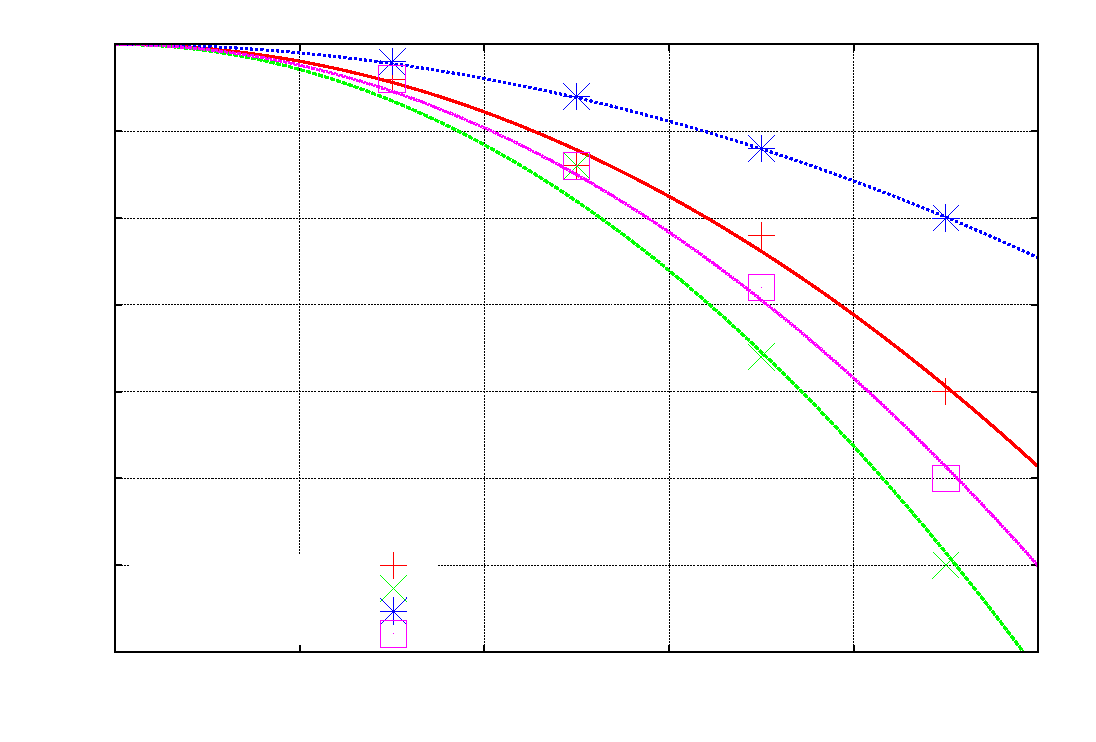
\includegraphics{vada}}%
    \gplfronttext
  \end{picture}%
\endgroup

\caption{Kulová vada tenké čočky. Vypuklá/ploská označuje, která strana čočky byla směrem k předmětu.}
\label{g:vada}
\end{graph}




Pomocí goniometru jsme změřili vzdálenost hlavních rovin. 
Polohy obou uzlových bodů jsme změřili víckrát, z hodnot jsme určili standardní odchylku a tu přenesli součtem čtverců do hodnoty $\delta$. Jednotlivé hodnoty jsou uvedeny v tabulce \ref{t:goniometr}. 
Celkové výsledky jsou
\begin{equation*}
\delta_{tenka} = \SI{12.9(3)}{\mm} \qquad \qquad \delta_{tlusta} = \SI{3.9(3)}{\mm}
\end{equation*}


\begin{tabulka}[htbp]
\centering
\begin{tabular}{c|cccc}
\multicolumn{5}{c}{Tenká čočka} \\
vypuklá & \SI{12.3}{\mm} & \SI{12.1}{\mm} & \SI{12.1}{\mm} & \\
ploská & \SI{16.0}{\mm} & \SI{15.7}{\mm} & \SI{16.3}{\mm} & \SI{16.2}{\mm} \\

\hline \hline
\multicolumn{5}{c}{Tlustá čočka} \\
vypuklá & \SI{13.7}{\mm} & \SI{13.2}{\mm} & \SI{13.3}{\mm} & \SI{13.3}{\mm} \\
ploská & \SI{26.1}{\mm} & \SI{26.2}{\mm} & \SI{26.5}{\mm} & \\
\end{tabular}
\caption{Měření vzdálenosti hlavních rovin pomocí goniometru. První sloupec označuje, která strana čočky byla směrem k okuláru, ostatní sloupce jsou poloha uzlového bodu na mikrometru.}
\label{t:goniometr}
\end{tabulka}



Na fokometru jsme změřili optickou mohutnost tenké čočky. Vypuklou stranou čočky k okuláru jsme změřili \SI{10.25(25)}{\per\metre}, ploskou stranou \SI{9.75(25)}{\per\metre}.


Tloušťka tlusté čočky byla \SI{38}{\mm}. Dosazením do \eqref{e:tlusta} jsme určili index lomu skla $n_{tlusta}=\num{1.51(3)}$.

%Diskuze výsledků
\section*{Diskuze}
Při měření kulové vady jsme považovali clonu č. 1 za paraxiální, tedy kulovou vadu pro ostatní clony jsme měřili jako rozdíl mezi polohami obrazu první a oné clony. Vzniklá chyba je zanedbatelná v porovnání s ostatními vlivy.

Podle zadání jsme považovali za $s$ aritmetický průměr vnějšího a vnitřního poloměru clony. K tomuto postupu není zřejmý důvod, jako lepší se jeví místo aritmetického průměru použít kvadratický průměr nebo ještě lépe $s$ středované přes intenzitu světla. Obraz bude v každém případě rozostřen a my neznáme přesný mechanismus vyhodnocování jeho polohy a nemůžeme tedy rozhodnout, která z možností je nejlepší. Proto předpokládáme, že použití aritmetického průměru má dobrý důvod a je správné.

Kulová vada je u obou předmětových vzdáleností větší, když je čočka orientovaná ploskou stranou k předmětu, což kvalitativně odpovídá našim výpočtům. Kulová vada je větší pro menší z obou předmětových vzdáleností.

Při Besselově metodě jsme se dopustili systematické chyby, protože jsme zanedbali tloušťku čočky. $D$ ve skutečnosti není vzdálenost vzdálenost předmětu a obrazu, ale $D=a+\apr$, kde $a$ a $\apr$ se měří od hlavních rovin. Abychom dostali správnou hodnotu $D$, musíme od změřené odečíst vzdálenost hlavních rovin $\delta_{tenka}$. Potom by vyšla ohnisková vzdálenost \SI{10.69(10)}{\cm}, tedy jsme se dopustili systematické chyby přibližně \SI{1.3}{\percent}.

Při metodě dvojího zvětšení je vnesená systematická chyba zanedbatelná. Výpočet ze změny obrazových vzdáleností byl přesnější. V každé dvojici má vždy buď součin $\beta_1\beta_2$ nebo rozdíl $\left|a_1-a_b\right|$ velkou chybu.

Rozmezí obou hodnot optické moutnosti, které jsme změřili na fokometru, přibližně odpovídá změřené optické vzdálenosti.

Metoda dvojího zvětšení byla přesnější.

Index lomu skla vypočtený z tloušťky tlusté čočky a vzdálenosti jejích hlavních rovin je v rozsahu hodnot, kterých běžně nabývá. Tabelovaná hodnota je 1,5-1,9.

%Závěr
\section*{Závěr}


\printbibliography[title={Seznam použité literatury}]

\end{document}